\documentclass{article}

\usepackage{amsmath}
\usepackage{amssymb}
\usepackage{hyperref}
\usepackage{url}
\usepackage{graphicx}
\usepackage{geometry}
\usepackage{enumitem}
\usepackage{parskip}
\usepackage{chemfig}
\usepackage{pdfpages}
\usepackage{xcolor}
\usepackage{tikz}
\usepackage{fancybox}
\usepackage{makecell}
\usepackage{pgfplots}
\usepackage{soul}
\usepackage{ulem}
\usepackage{wrapfig}
\usepackage{subcaption}
\usepackage[T1]{fontenc}
\usepackage{esvect}
\usepackage{multirow}
\usepackage{booktabs}
\usepackage{float}
\usepackage{tocloft}
\usepackage{caption}
\usepackage{colortbl}
\usepackage{siunitx}
\usepackage{footnote}
\usepackage{listings}
\usetikzlibrary{arrows}
\usetikzlibrary{decorations.pathreplacing}
\pgfplotsset{compat=1.17}
\usepgfplotslibrary{statistics}
\definecolor{darkgray}{rgb}{0.2, 0.2, 0.2}

% === BIBLIOGRAPHY ===
\usepackage[utf8]{inputenc}
\usepackage{csquotes}
\usepackage[style=apa,citestyle=numeric,backend=biber]{biblatex}
\addbibresource{ref.bib}
\DeclareFieldFormat[article]{volume}{\textbf{#1}}
\DeclareFieldFormat[article]{journaltitle}{\textit{#1}}

% ----- OPTIONAL -----
\DeclareFieldFormat{labelnumberwidth}{\mkbibbrackets{#1}}
\defbibenvironment{bibliography}
  {\list
     {\printfield[labelnumberwidth]{labelnumber}}
     {\setlength{\labelwidth}{\labelnumberwidth}%
      \setlength{\leftmargin}{\labelwidth}%
      \setlength{\labelsep}{\biblabelsep}%
      \addtolength{\leftmargin}{\labelsep}%
      \setlength{\itemsep}{\bibitemsep}%
      \setlength{\parsep}{\bibparsep}}%
      \renewcommand*{\makelabel}[1]{##1}}
  {\endlist}
  {\item}
% ====================
 
\geometry{
    a4paper,
    total={170mm, 257mm},
    left=20mm,
    top=20mm
}

\hypersetup{
    colorlinks=true,
    linkcolor=black,
    urlcolor=blue,
    pdftitle={Report SW10 - EnCheBio}
}

\newcommand{\figbox}[1]{ 
    \begin{figure*}[ht!]        
        \begin{center}            
            \fbox{#1}        
        \end{center}    
    \end{figure*}
}

\newcommand{\wrapfill}{
    \par
    \ifnum \value{WF@wrappedlines} > 0
        \addtocounter{WF@wrappedlines}{-1}%
        \null\vspace{
            \arabic{WF@wrappedlines}
            \baselineskip
        }
        \WFclear
    \fi
    \phantom{}
}

\newcommand{\cfig}[3]{
    \centering
    \chemfig{#1}
    \captionof{figure}{#3}
    \label{#2}
}


% === LIST OF EQUATIONS ===
\newcounter{myequation}
\renewcommand{\themyequation}{\arabic{myequation}}

\newlistof{myequations}{loe}{\Large List of Equations}
\newcommand{\addequationtotoc}[1]{\addcontentsline{loe}{myequations}{\protect\numberline{\themyequation}#1}}

\renewcommand{\cftmyequationspresnum}{}
\renewcommand{\cftmyequationsaftersnum}{\hspace{1em}}
\setlength{\cftmyequationsnumwidth}{2em}
\cftsetindents{myequations}{1.5em}{2.3em}

\newcommand{\capeq}[3]{
    \refstepcounter{myequation}
    \begin{equation*}
        #1
    \end{equation*}
    \label{#2}
    \begin{center}
        \vspace*{-.4cm}
        \noindent{Equation \themyequation:} #3
    \end{center}
    \addequationtotoc{#3}
}

\newcommand{\refeq}[1]{\hyperref[#1]{Equation~\ref*{#1}}}
% =========================

\newcommand{\difference}{\,\backslash\,}
\newcommand{\rem}{\underline{Remark}: }
\newcommand{\nots}{\underline{Notation}: }
\newcommand{\prf}{\underline{Proof}: }
\newcommand{\exs}{\underline{Example}: }
\newcommand{\defs}{\underline{Definition}: }
\newcommand{\wrn}{\underline{Warning}: }
\newcommand{\sht}{\ |\ }
\newcommand{\pph}[1]{\paragraph{#1}\phantom{}\\}
\newcommand{\dm}{\displaystyle}

\newcommand{\ccit}[1]{\citeauthor{#1} \cite{#1}}

\lstset{
    basicstyle=\ttfamily\footnotesize,
    keywordstyle=\color{blue}\bfseries,
    commentstyle=\color{green!60!black},
    stringstyle=\color{red},
    showstringspaces=false,
    numbers=left,
    numberstyle=\tiny,
    frame=single,
    breaklines=true
}

% === TEXT ===
\begin{document}

\hypersetup{citecolor=black}

\begin{minipage}{0.7\textwidth}
    \vspace*{-.8cm} \hspace*{-0.3cm}
    \includegraphics[width=.5\textwidth]{media/hslu-logo.png}
\end{minipage}

\vspace*{2cm}

\textbf{\huge Practical 3:}\\[.75cm]
\begin{center}
    \textbf{\huge Analysis of PAHs in Plastics}
    
    \textbf{\huge by GC-MS}\\[1cm]
    
    \includegraphics[width=\textwidth]{media/front_practical3.png}\\
\end{center}

\vfill

\setlength{\intextsep}{0pt}%
\begin{wrapfigure}{r}{\textwidth}
    \textbf{\Large Environmental Chemistry and Biology HS2024\\[.5cm]
    \large Dr. Macarena San Martín Ruiz\\
    Lecturer}
    \vspace{-2.1cm}
\end{wrapfigure}

\phantom{}\\[-1cm]

\begin{flushright}
        \large
        \textbf{Team 4}\\
        Matteo Frongillo\\
        Ramadhan Nura\\
        Folagbade Popoola\\
        Jonathan Lawrence Boms\\
        Kron Xhemajli
\end{flushright}
\wrapfill
\newpage
\tableofcontents
\pagebreak

\section{Introduction}
The purpose of this experiment is to analyze and quantify polycyclic aromatic hydrocarbons
(PAHs) in plastics using Gas Chromatography-Mass Spectrometry (GC-MS). PAHs are a group of
organic compounds consisting of multiple aromatic rings and are commonly found as
contaminants in the environment due to incomplete combustion of organic matter. Since PAHs
pose significant risks to human health and the environment, their detection and
quantification are critical in environmental chemistry.

This experiment introduces key analytical techniques, such as chromatographic separation
based on molecular properties (e.g., boiling points and hydrophobicity) and mass
spectrometric detection of characteristic ion fragments. Calibration curves and internal
standards are also employed to ensure accurate quantification of the detected PAHs.

\subsection{PAHs}
Polycyclic Aromatic Hydrocarbons (PAHs) are a group of organic compounds composed of
multiple aromatic rings made up of carbon and hydrogen atoms. They are primarily formed as
byproducts of incomplete combustion of organic matter. PAHs are widespread in the
environment and can be found in air, soil, water, and food sources. Common sources
include vehicle emissions, industrial processes, and natural events like wildfires.

The detection of PAHs is of great importance due to their potential adverse effects on
human health and the environment. Many PAHs are known to be carcinogenic, mutagenic, and
toxic, posing serious risks through prolonged exposure. They can accumulate in the food
chain, contaminating water supplies and agricultural produce. As a result, monitoring and
quantifying PAHs in various matrices, such as plastics, soil, and water, are essential for
assessing pollution levels, mitigating environmental contamination, and ensuring public
health safety. Analytical techniques like GC-MS allow for accurate identification and
quantification of PAHs, providing critical data for regulatory purposes and environmental
management.

\section{Materials and Methods}
\subsection{Materials}
\begin{itemize}
    \item Gas chromatograph -- Mass spectrometer
    \item Helium (carrier gas)
    \item Standard PAH kit
    \item Chloroform (solvent)
    \item Vials
    \item Pipettes
\end{itemize}

\subsection{Procedure}
In this experiment, a standard solution of PAHs was initially prepared by diluting the
stock solution to achieve a concentration ratio of 1:10 in chloroform. To ensure accuracy
and precision during the preparation process, calibrated syringes were used to carefully
measure the required volumes. For the subsequent dilution to 1:100, 0.9 mL of the 1:10
solution was precisely transferred into a clean vial using a syringe, minimizing any
possible errors in volume measurement. The remaining volume was then filled with
chloroform to achieve a final solution volume of 1 mL, ensuring consistent and accurate
preparation of the diluted sample. The proper use of syringes and sealing techniques
contributed to the reliability and reproducibility of the experimental results.

Once the dilution process was complete, the vial was tightly sealed using specialized caps
to prevent contamination or solvent evaporation, which could affect the sample integrity
and analysis. These sealed vials were then carefully handled and introduced into the Gas
Chromatography-Mass Spectrometry (GC-MS) system for analysis.

\subsection{Preparation of diluted solutions for a calibration curve}
\subsubsection{Legend}
\begin{itemize}
    \item $\mathbf{C_i}$: Initial stock concentration ($\mu$g/mL)
    \item $\mathbf{C_t}$: Target concentration ($\mu$g/mL)
    \item $\mathbf{V_s}$: Volume of stock solution required (mL)
    \item $\mathbf{V_t}$: Target volume (mL)
    \item $\mathbf{V_c}$: Volume of chloroform required (mL)
\end{itemize}

\subsubsection{Formulas}
\begin{itemize}
    \item Amount of volume of stock solution required $\mathbf{V_s}$:
    \capeq{V_s = \frac{C_t \cdot V_t}{C_i}}{eq:vol_stock}{Stock solution volume}
    \item Volume of chloroform required $\mathbf{V_c}$:
    \capeq{V_c = V_t - V_s}{eq:vol_solvent}{Solvent volume}
\end{itemize}

\subsubsection{Ratios}
\begin{table}[H]
    \centering
    \caption{Diluted solution ratios}
    \begin{tabular}{@{}lcllcl@{}}
        \toprule
        \textbf{Dilution} & $\mathbf{C_i}$ & $\mathbf{C_t}$ & $\mathbf{V_s}$ & $\mathbf{V_t}$ & $\mathbf{V_c}$\\
        \midrule
        1:10 & 10 & 1 & 0.1 & 1 & 0.9\\
        1:100 & 10 & 0.1 & 0.01 & 1 & 0.99\\
        1:1000 & 10 & 0.01 & 0.001 & 1 & 0.999\\
        \bottomrule
    \end{tabular}
    \label{tab:ratios}
\end{table}

\newpage
\section{Results}
\subsection{Chromatogram}
\vspace*{.5cm}
\begin{figure}[ht!]
    \centering
    \includegraphics[width=\textwidth]{media/cg/cg.png}
    \label{fig:chromatogram}
    \caption{Chromatogram}
\end{figure}
\vspace*{.5cm}
The GC-MS chromatogram reveals the PAHs detected in the chromatography experiment.
Each peak corresponds to a specific compound separated based on its retention time.
The x-axis represents retention time (minutes), while the y-axis shows the relative
abundance (intensity) of the detected compounds.

The graph displays several distinct peaks, where the height of each peak reflects the
intensity of the signal generated by the detector, which is proportional to the compound's
concentration. The retention time of each peak increases from left to right, indicating
that compounds with higher boiling points and greater hydrophobicity elute later from the
column.
\vspace*{.5cm}
\subsubsection{Data analysis}
\begin{table}[ht!]
    \centering
    \caption{Compounds data}
    \begin{tabular}{@{}llcllcc@{}}
        \toprule
        \textbf{Nr.} & \textbf{Compound} & \textbf{Concentration} & \textbf{Retention} & \textbf{Peak area} & \textbf{m/z} & \textbf{RF}\\
        & \textbf{name} & \textbf{(ng/mL)} & \textbf{time} & & \textbf{fragments}\\
        \midrule
        1 & \nameref{ch:naphthalene} & 1000 & 4.62 & 938975 & 128 & 939\\
        2 & \nameref{ch:acenaphthylene} & 1000 & 7.78 & 1093694 & 152 & 1094\\
        3 & \nameref{ch:acenaphthene} & 1000 & 8.18 & 1306917 & 154 & 1307\\
        4 & \nameref{ch:fluorene} & 1000 & 9.35 & 1134899 & 166 & 1135\\
        5 & \nameref{ch:anthracene} & 1000 & 11.58 & 1115451 & 178 & 1115\\
        6 & \nameref{ch:phenanthrene} & 1000 & 11.71 & N.D. & 178 & N.D.\\
        7 & \nameref{ch:pyrene} & 1000 & 14.46 & 1358324 & 202 & 1358\\
        8 & \nameref{ch:fluoranthene} & 1000 & 15.00 & 1533223 & 202 & 1533\\
        9 & \nameref{ch:chrysene} (1) & 1000 & 18.08 & 133907 & 114 & 134\\
        10 & \nameref{ch:chrysene} (2) & 1000 & 18.21 & 992122 & 228 & 992\\
        \bottomrule
    \end{tabular}
    \label{tab:calibration-data}
\end{table}
\vspace*{.5cm}
The table summarizes the key results from the GC-MS analysis, listing the detected PAHs,
their retention times, peak areas, and m/z fragments.

\newpage
\pph{Data interpretation}
Retention time increases progressively from 4.62 min to 18.21 min in correlation with
increasing molecular weight and complexity of the compounds.

Naphthalene elutes first due its lower molecular weight and boiling point, while Chrysene (2)
elutes later, consistent with its higher boiling point and hydrophobicity.

\pph{Peak area}
The peak area reflects the relative abundance of each compound in the sample.

Compounds like Fluoranthene and Pyrene show high peak areas, indicating higher concentrations.
In contrast, Chrysene (1) has a significantly lower peak area, suggesting a lower relative
abundance.

\pph{m/z fragments}
The m/z values provide confirmation of the molecular identity of each compound.

Naphthalene shows m/z = 128, corresponding to its molecular ion, and Chrysene (2) shows
m/z = 228, consistent with its larger structure and molecular weight.

\pph{Response factor (RF)}
The RF values indicate the sensitivity of the detector to each compound. Higher RF values
suggests stronger signal responses, while lower values may reflect weaker detection efficiency.

\subsection{PAHs detected}
\subsubsection{LMW PAHs}
Low Molecular Weight PAHs exhibited lower retention times due to their smaller molecular 
weights and lower boiling points.

\noindent
\begin{minipage}{0.32\textwidth}
\cfig{[:0]*6(=-*6(-=-=-)=-=-)}{ch:naphthalene}{Naphthalene}
\end{minipage}%
\begin{minipage}{0.32\textwidth}
\cfig{[:0]*6(=-*6(-=-=(-[:112]-[:180]-[:249 ])-)=-=-)}{ch:acenaphthene}{Acenaphthene}
\end{minipage}%
\begin{minipage}{0.32\textwidth}
\cfig{[:0]*6(=-*6(-=-=(-[:112]=[:180]-[:249 ])-)=-=-)}{ch:acenaphthylene}{Acenaphthylene}
\end{minipage}

\vspace{0.5cm}

\noindent
\begin{minipage}{0.32\textwidth}
\cfig{*6(=-(*5(-(*6(-=-=-=))----))=-=-)}{ch:fluorene}{Fluorene}
\end{minipage}%
\begin{minipage}{0.32\textwidth}
\cfig{*6(=-(*6(-(*6(-=-=--))=-=-))=-=-)}{ch:phenanthrene}{Phenanthrene}
\end{minipage}%
\begin{minipage}{0.32\textwidth}
\cfig{*6(=-(*6(-=(*6(-=-=--))-=--))=-=-)}{ch:anthracene}{Anthracene}
\end{minipage}

\newpage
\subsubsection{HMW PAHs}
High Molecular Weight PAHs were identified at longer retention times. These compounds are
characterized by their larger molecular structures and higher boiling points.

\noindent
\begin{minipage}{0.32\textwidth}
\cfig{*6(-=(*6(-=-(*6(-(*6(-=-=--))=-=--))=--))-=-=)}{ch:chrysene}{Chrysene}
\end{minipage}%
\begin{minipage}{0.32\textwidth}
\cfig{*6(-=(*6(-=-=(-[:112]([:120]*6(-=-=-=))-[:180]-[:249])--))-=-=)}{ch:fluoranthene}{Fluoranthene}
\end{minipage}%
\begin{minipage}{0.32\textwidth}
\cfig{*6(=-(*6(-=-=--))=(*6(--=---))-(*6(=-=-=-))--)}{ch:pyrene}{Pyrene}
\end{minipage}

\section{Discussion}
\subsection{Questions}
\subsubsection{Question 1}
\begin{enumerate}
    \item According to the chemical structures, hydrophobicity and boilind points, which compound
    will appear first in the GC chromatogram?

    \textbf{R:} Naphthalene elutes first.

    \item Which compound will appear last?
    
    \textbf{R:} Benzo(g,h,i)perylene elutes last.

    \item Explain why in a few sentences.

    \textbf{R:}\\
    Compounds separate and elute based on their physical and chemical properties,
    primarily their boiling points and hydrophobicity.
    Hydrophobicity refers to a compound's tendency to repel water and interact with
    non-polar environments, increasing with the number of aromatic rings due to enhanced
    molecular stability and larger surface areas.
    Similarly, boiling point rises with more aromatic rings because of stronger
    intermolecular forces.

    These properties allow them to travel through the GC column more
    quickly, resulting in shorter retention times and earlier elution in the chromatogram.
    (\ccit{restek1}).

    \newpage
    \item Consider the chemical structure of naphthalene. Which fragments will be visible
    in the MS spectrum?

    \textbf{R:}
    In the mass spectrum of naphthalene, the following fragments are commonly observed\footnotemark:
    \begin{itemize}
        \item Molecular ion (M$^+$), which corresponds to the intact naphthalene molecule
            with a single positive charge (m/z = 128);
        \item Fragment ions, which are ionization results in the loss of hydrogen atoms
            (m/z = 127 for the loss of one hydrogen atom);
        \item Smaller hydrocarbon fragments, which include common fragmet from cleavage
            of the aromatic ring (like m/z = 63).
    \end{itemize}
    \footnotetext{Source: \ccit{libretexts}, \ccit{naphthalene}}

    \vspace*{.3cm}
    \begin{figure}[ht!]
        \centering
        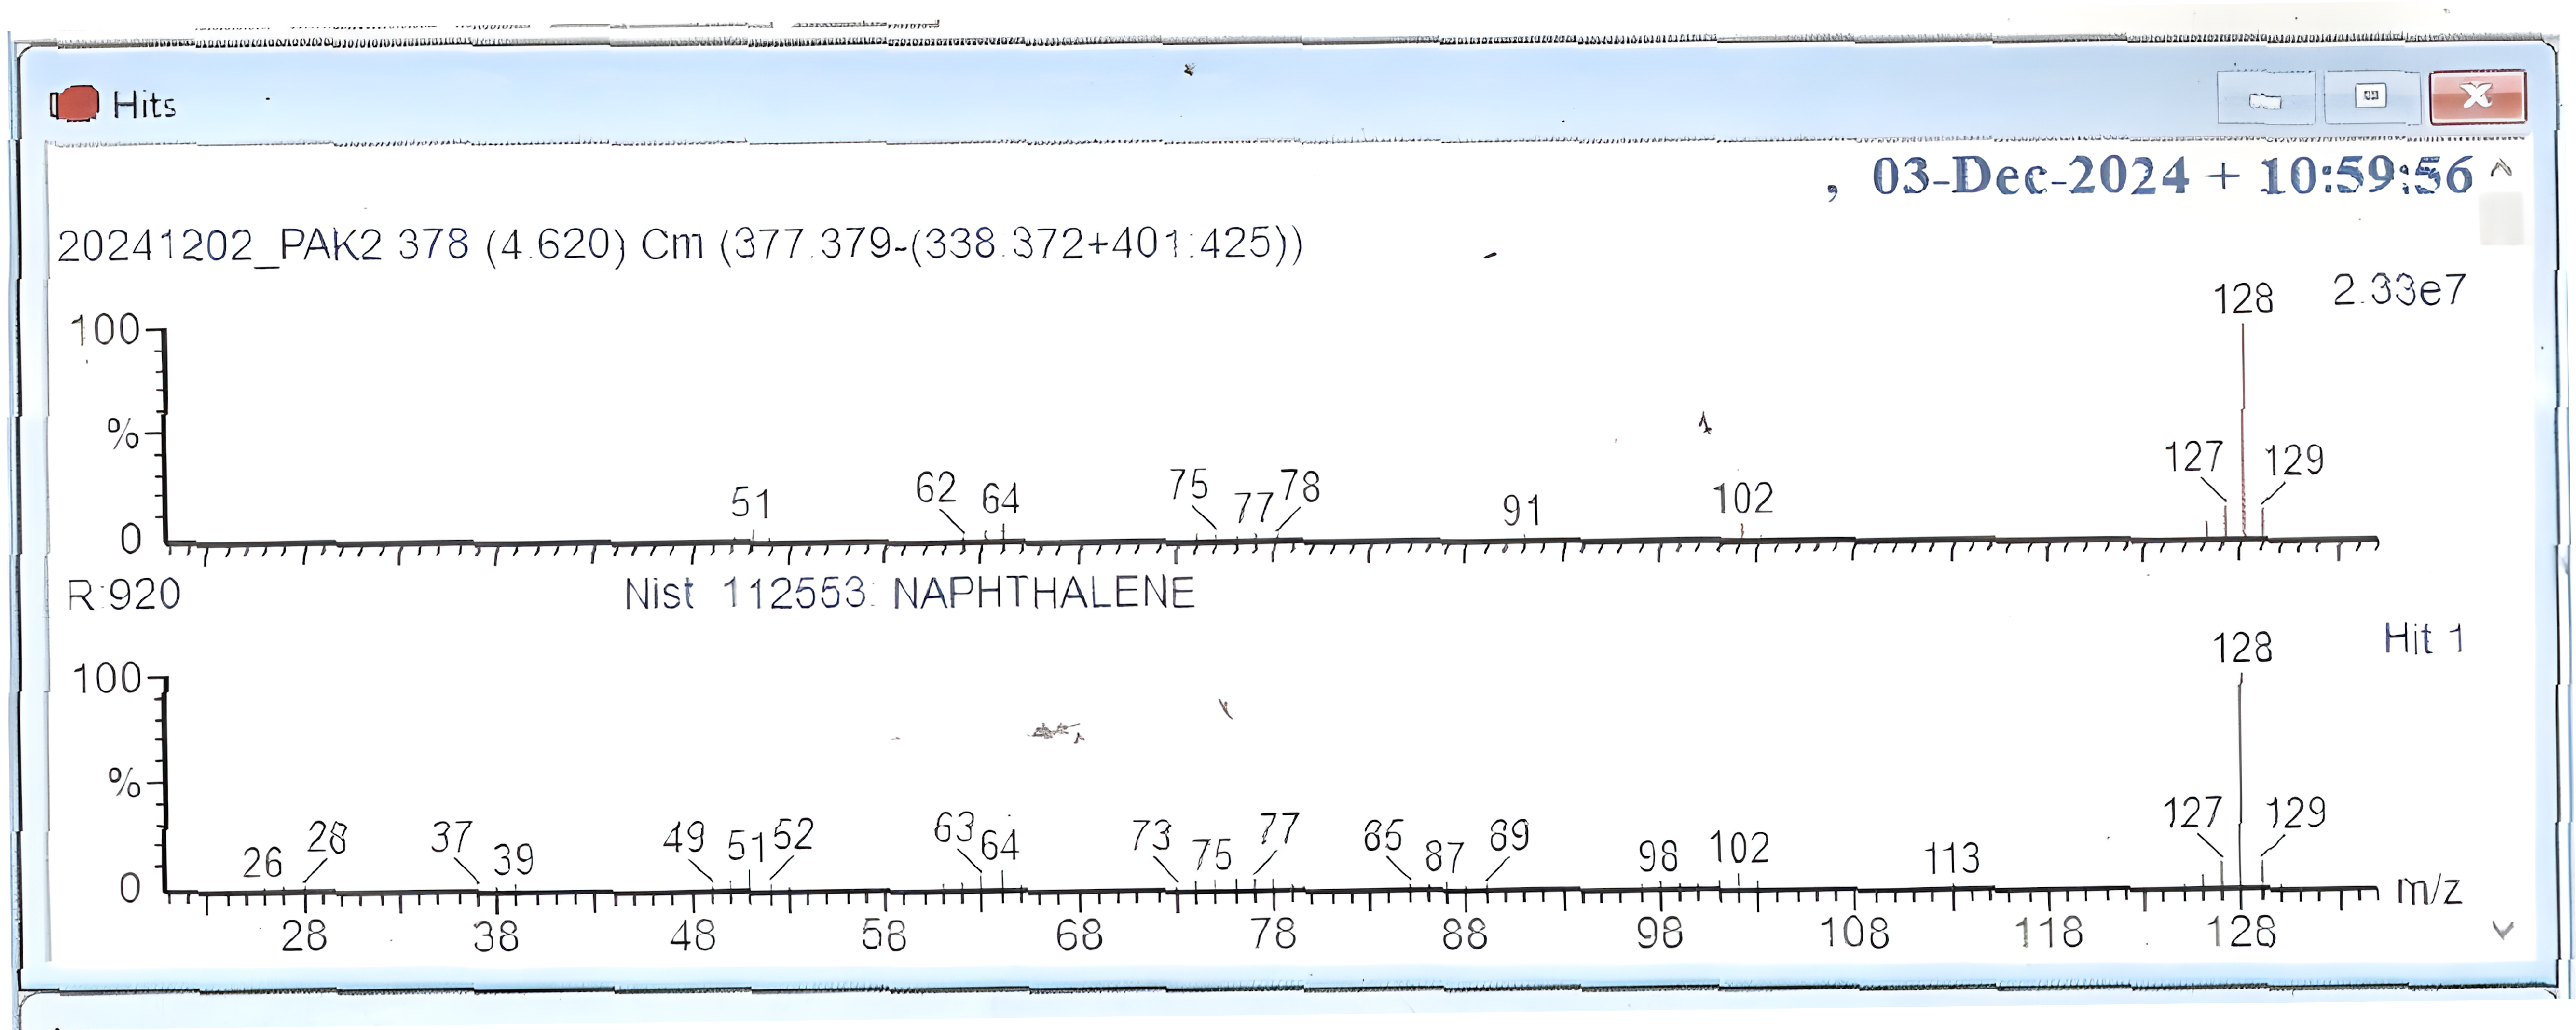
\includegraphics[width=.7\textwidth]{media/cg/mz.png}
        \label{fig:m/z}
        \caption{Naphthalene m/z fragments}
    \end{figure}
    \vspace*{.5cm}

    \item Can you predict the order of appearance in the GC chromatogram for all PAHs?
    \vspace*{.5cm}
    \begin{table}[H]
        \centering
            {\footnotesize}
            \caption{PAHs order of appearance}
        \begin{tabular}{@{}clcc@{}}
            \toprule
            \textbf{Order of} & \textbf{Compound} & \textbf{Rings} & \textbf{Boiling point}\footnotemark\\
            \textbf{appearance} & \textbf{name} & \textbf{nr.} & \textbf{($^\circ$C)}\\
            \midrule
            1 & Naphthalene & 2 & 218\\
            2 & Acenaphthene & 3 & 278\\
            3 & Acenaphthylene & 3 & 280\\
            4 & Fluorene & 3 & 294\\
            5 & Phenanthrene & 3 & 338\\
            6 & Anthracene & 3 & 342\\
            7 & Fluoranthene & 4 & 384\\
            8 & Pyrene & 4 & 404\\
            9 & Benzanthracene & 4 & 438 \\
            10 & Chrysene & 4 & 448\\
            11 & Benzo(k)fluoranthene & 5 & 480\\
            12 & Benzo(b)fluoranthene & 5 & 481\\
            13 & Benzo(a)pyrene & 5 & 496\\
            14 & Dibenzo(a,h)anthracene & 5 & 524\\
            16 & Indeno(c,d)pyrene & 6 & 536\\
            16 & Benzo(g,h,i)perylene & 6 & 550\\
            \bottomrule
        \end{tabular}
        \label{tab:gc-appearance}
    \end{table}
    \footnotetext{Source: \href{https://pubchem.ncbi.nlm.nih.gov/}{PubChem} \cite{pubchem}}
\end{enumerate}
\vfill

\newpage
\subsubsection{Question 2}
Chrysene, a 4-ring PAH, is detected in an environmental water sample using GC-MS. The
concentration of Chrysene in the sample must be calculated! Calculate the concentration
with two method:
\pph{1. The calibration curve method}
A set of samples with known concentration of Chrysene were measured and gave the
following result in the chromatogram:
\vspace{.5cm}
\begin{figure}[ht!]
    \centering
    \includegraphics[width=.8\textwidth]{media/question_2.1.png}
    \label{fig:question_2.1}
    \caption{Chrysene samples CG-measurements}
\end{figure}

\textbf{Formulas}:
\begin{itemize}
    \item Calibration curve with linear regression:
    \capeq{A=mx+b}{eq:cal_curve}{Calibration curve}
    where:\\
    $A$ = peak area\\
    $m$ = slope of the line\\
    $x$ = concentration\\
    $b$ = y-intercept

    \item Concentration measurement ($x$):
    \capeq{x = \frac{A-b}{m}}{eq:unknown_sample}{Concentration of the unknown sample}
\end{itemize}

The unknown sample of Chrysene gave the following result: Peak Area = 300 a.u.;

Calculate the concentration of the unknown sample:

\textbf{R:}

The slope has been calculated with a Python script (\ref{sec:linear_python})
using the following formula:
\capeq{m=\frac{\sum x\cdot y}{\sum x^2}}{eq:slope}{Calibration curve slope}

\newpage
With this script, which forces the function to pass by the point (0,0), a slope of $m=5.14$
is obtained.

\vspace*{.5cm}
\begin{figure}[h!]
    \centering
    \begin{tikzpicture}
    \begin{axis}[
        width=12cm,
        height=8cm,
        xlabel={Concentration (ng/mL)},
        ylabel={Peak Area (a.u.)},
        grid=both,
        legend pos=north west,
        legend style={font=\small},
        legend cell align={left},
    ]

    \addplot[
        domain=0:220,
        samples=500,
        thick,
        color=black
    ] {5.143396226415095 * x};
    \addlegendentry{$y = 5.14x$}

    \addplot[only marks, mark=*, color=blue] coordinates {
        (10, 50) (20, 105) (50, 260) (100, 520) (200, 1025)    
    };
    \addlegendentry{Data points}
    
    \end{axis}
    \end{tikzpicture}
    \caption{Chrysene calibration curve}
    \label{fig:tap_ph}
\end{figure}
\vspace*{.5cm}

\textbf{Calculation}:

Calculating the concentration of chrysene with $A=300$ a.u., according to the \refeq{eq:unknown_sample},
we obtain:
\vspace*{.5cm}
\figbox{$\dm x = \frac{300 \text{ a.u.} - 0}{5.14} = 58.33 \text{ ng/mL}$}

\newpage
\pph{2. The internal standard method}
An internal standard, Fluoranthene, was injected in the unknown Chrysene sample with
concentration 50 ng/mL. The following chromatogram was obtained:
\vspace*{.5cm}
\begin{figure}[ht!]
    \centering
    \includegraphics[width=.8\textwidth]{media/question_2.2.png}
    \label{fig:question_2.2}
    \caption{Unknown sample and Chrysene chromatogram}
\end{figure}

\textbf{Formulas:}
\begin{itemize}
    \item Response factor of the sample \textbf{RF}:
    \capeq{RF = \frac{\text{Peak area}}{\text{Concentration}}}{eq:response_factor}{Response factor}
    \item Relative response factor of the sample \textbf{RF$\mathbf{_{rel}}$}:
    \capeq{RF_{\mathbf{rel}} = \frac{\text{RF analyte}}{\text{RF internal standard}} = \frac{\frac{\text{Peak area of analyte}}{\text{unknown concentration of analyte}}}{\frac{\text{Peak area of internal standard}}{\text{concentration of internal standard}}}}{eq:rel_response_factor}{Relative response factor}
    \item Concentration of the unknown sample (x):
    \capeq{x = \frac{\text{peak of analyte} \cdot \text{concentration of internal standard}}{\text{peak area of internal standard} \cdot \text{relative RF}}}{eq:unknown_concentration}{Unknown concentration of analyte}
\end{itemize}

Based on the data provided, calculate the concentration of Chrysene in the sample:

\textbf{R}:

Assuming that \underline{$RF_{\text{rel}} = 1$}, then:
\figbox{$\dm x = \frac{300 \text{ a.u.} \cdot 50 \text{ ng/mL}}{500 \text{ a.u.} \cdot 1} = 30 \text{ ng/mL}$}

\newpage
\section{Conclusion}
\subsection{Summary of the experiment}
This experiment successfully demonstrated the application of Gas Chromatography-Mass
Spectrometry (GC-MS) for the analysis and quantification of polycyclic aromatic
hydrocarbons (PAHs) in plastic samples. The chromatographic separation provided clear
identification of individual PAHs based on retention times, which increased with the
molecular weight and complexity of the compounds. The mass spectrometry data, including
characteristic m/z fragments, validated the molecular identity of the detected compounds,
such as naphthalene and chrysene, aligning with theoretical expectations.

\subsection{Calibration curve and quantification}
The calibration curve approach showed high linearity. Using this method, the unknown
concentration of chrysene in the sample was accurately determined as 58.33 ng/mL.
Additionally, the internal standard method, incorporating fluoranthene, provided a
secondary verification with a calculated chrysene concentration of 30 ng/mL, emphasizing
the utility of complementary techniques to enhance data robustness.

\subsection{PAHs separation}
The results revealed the clear separation between low molecular weight (LMW) and high
molecular weight (HMW) PAHs. Compounds with fewer aromatic rings eluted earlier due to
lower boiling points and hydrophobicity, while larger PAHs required longer retention times.
This trend was consistent with the expected behavior of PAHs during chromatographic
separation.

\subsection{PAHs mitigation}
Mitigating the presence of polycyclic aromatic hydrocarbons (PAHs) in the environment is
crucial due to their carcinogenic and toxic effects. Effective strategies include reducing
emissions from industrial processes, vehicles, and other combustion sources by adopting
cleaner technologies and fuels. Additionally, remediation techniques such as
bioremediation, which employs microorganisms to degrade PAHs, have shown promising results
in contaminated soils and waters.

Regulatory measures also play a vital role in mitigation. Enforcing stricter emission
standards and monitoring programs can help limit PAH release into the environment.
Recycling and proper disposal of materials containing PAHs, like plastics, further
contribute to minimizing environmental contamination. Public awareness campaigns and
industrial compliance with environmental regulations are essential for the long-term
reduction of PAHs, ensuring both environmental and human health protection \ccit{HARITASH20091}.

\newpage
\listoffigures

\listoftables

\listofmyequations

\setlength{\bibitemsep}{1.2\baselineskip}
\printbibliography

\newpage
\section{Attachments}
\subsection{Question 2.1}
\label{sec:linear_python}
Python script for the linear regression:

\begin{lstlisting}[language=Python, caption=Calibration curve]
    import numpy as np

    x = np.array([10, 20, 50, 100, 200])
    y = np.array([50, 105, 260, 520, 1025])
    
    slope = np.sum(x * y) / np.sum(x**2)
    
    print("slope:", slope)
    print("300/slope:", 300/slope)
\end{lstlisting}

Output:
\begin{lstlisting}
    slope: 5.143396226415095
    300/slope: 58.32721936903888
\end{lstlisting}

\end{document}